\section{The algorithm C2-AS-FI}
\label{sec:C2-AS-FI}

The most expensive step of C2-AS is the polynomial interpolation step
which is part of the Cauchy interpolation. If we use a standard
interpolation algorithm, its input consists in a list of $\Theta(p^k)$
pairs $\bigl(P, \I(P)\bigr)$, with $P$ having coordinates in $\U_k$,
thus a lower bound for any such algorithm is $\Omega(p^{2k}d)$. Notice
however that the output is a polynomial of degree $\Theta(p^k)$ in
$\F_q[X]$, hence, if supplied with a shorter input, an \emph{ad hoc}
algorithm could reach the bound $\Omega(p^kd)$.

In this section we give an algorithm that reaches this bound up to
some logarithmic factors. It realizes the polynomial interpolation on
the primitive points of $E[p^k]$, thus its output is a degree
$\euler(p^k)/2-1$ polynomial in $\F_q[X]$. Using the Chinese remainder
theorem it is straightforward to generalize this to an algorithm,
having the same asymptotic complexity, that realizes the polynomial
interpolation on all the points of $E[p^k]$. We call C2-AS-FI the
variant of C2-AS resulting from applying this new algorithm.


\subsection{The algorithm}
Let $P\in E[p^k]$ and $P'\in E'[p^k]$ be primitive $p^k$ torsion
points. We want to compute the polynomial $A\in\F_q[X]$ such that
\begin{equation}
  A\bigl(x\bigl([n]P\bigr)\bigr) = x\bigl([n]P'\bigr)
  \quad\text{for any $n\in\left(\Z/p^k\Z\right)^\ast$.}
\end{equation}
As we saw in Section~\ref{todo}, such a polynomial is only defined
modulo the polynomial vanishing on the interpolation points
\begin{equation}
  T(X) = \prod_{n\in\left(\Z/p^k\Z\right)^\ast} \bigl(X - x([n]P)\bigr)
  \text{.}
\end{equation}
Thus we look for the canonical representative of $A$ in $\F_q[X]/T(X)$.

We start by applying the Chinese remainder theorem to $\F_q[X]/T(X)$:
let
\begin{equation}
  \label{eq:T}
  T = \prod T^{(j)}
\end{equation}
be the factorization of $T$ over $\U_0$, and set
\begin{equation}
  \label{eq:A}
  A^{(j)} \eqdef A \bmod T^{(j)}
  \;\text{.}
\end{equation}
Define
\begin{equation}
  \label{eq:187}
  \K_j\eqdef\F_q[X]/T^{(j)}(X)  
  \text{,}
\end{equation}
then $\K_j$ is a field and $A^{(j)}$ is the projection of $A$ in
$\K_j$.

It was already pointed out in \cite[$\S$2.3]{couveignes96} that,
knowing the factorization of $T$ over $\U_0$ and all the $A^{(j)}$'s,
we can recover $A$ using the Chinese remainder algorithm. Thus we will
focus on computing, say, $A^{(0)}$.

Chose any root $\zeta$ of $T^{(0)}$, without loss of generality we
can take $\zeta=x(P)$, then
\begin{equation}
  \label{eq:188}
  \basis{B}=\{1,\zeta,\ldots,\zeta^{d-1}\}  
\end{equation}
is an $\F_q$-basis of $\K_0$.  Fix the $\F_q$-linear embedding of
finite fields
\begin{equation}
  \label{eq:embed}
  \xymatrix{
    \K_0 \ar@{^{(}->}[r]^-\iota & \U_k
  }
\end{equation}
given by $\iota(\zeta) = x(P)$, by linearity it is evident that
\begin{equation}
  \iota\bigl(A^{(0)}(\zeta)\bigr) = A^{(0)}\left(\iota(\zeta)\right)=x\bigl(P'\bigr)
  \text{.}
\end{equation}
Thus $\iota^{-1}\bigl(x(P')\bigr)$ is in $\K_0$ and the coefficients
of $A_0$ are its coordinates on the basis $\basis{B}$. In conclusion,
computing $A_0$ is equivalent to find a \hyperref[eq:22]{rational
  univariate representation} of $x(P')$ with respect to $x(P)$.

Unfortunately, applying algorithm RUR is not optimal: the bottleneck
is the power projection $\proj_\zeta$ appearing in
step~\ref{alg:rur:1}. We have seen in
Section~\ref{sec:shoups-algorithm} that the dual problem to power
projection is polynomial evaluation, thus in particular
\begin{equation}
  \label{eq:189}
  \begin{aligned}
    \dual{\proj_\zeta} = \ev_\zeta : \F_q[X] &\ra \K_j\text{,}\\
    g &\mapsto g(\zeta)\text{;}
  \end{aligned}
\end{equation}
so that any algorithm to evaluate polynomials at $\zeta$ yields a
power projection algorithm having the same complexity, and
\emph{vice-versa}. But none of the algorithms of
Chapter~\ref{cha:artin-schr-towers} allows to evaluate polynomials in
$\F_q[X]$ at a generic point of $\U_k$, better than a Horner rule.

We shall thus give an alternative algorithm to compute the minimal
polynomial $T_0$ of $x(P)$. It will be similar to a
\hyperref[todo]{subproduct tree}, but it will exploit the structure of
the Artin-Schreier tower. This is similar to the way we solved
Artin-Schreier equations in Section~\ref{sec:couveignes-algorithm}.


\paragraph{Interpolation in towers of extensions}
We set $\U_0=\F_q$. The algorithm we give here can be applied in any
tower of cyclic extensions, provided the action of the Galois groups
can be computed. However we will present it only for our specific
tower $(\U_0,\dots,\U_k)$, to avoid adding unnecessary notation.

Consider the following problem: given elements $x,y\in\U_k$ such that
$x$ generates $\U_k$ over $\F_q$, find a polynomial $A\in\F_q[X]$ such
that
\begin{equation}
  \label{eq:affine-minimal}
  A(x) = y
  \text{.}
\end{equation}
Let $T$ be the minimal polynomial of $x$ over $\F_q$, then, as above,
the class of $A$ in $\F_q[X]/T(X)$ is uniquely determined.

Let $A$ be a polynomial satisfying \eqref{eq:affine-minimal} it is
clear that $A(\sigma(x)) = \sigma(y)$ for any
$\sigma\in\Gal(\U_k/\F_q)$. Conversely, the polynomial interpolating
$\sigma(x)$ over $\sigma(y)$ for any $\sigma$ is invariant under
$\Gal(\U_k/\F_q)$, thus it has coefficients in $\F_q$. Hence we can
construct $A$ by interpolation.

A \hyperref[todo]{fast interpolation algorithm} would compute $T$ via
a binary subproduct tree, and then interpolate $A$ recursively
applying the Chinese remainder theorem along the branches of the
tree. However this is too expensive. We can do better by using a
non-binary subproduct tree on which the tower of Galois groups
associated to $(\U_0,\ldots,\U_k)$ acts.

First we need to compute $T$. Let $T_i$ be the minimal polynomial of
$x$ over $\U_i$, we compute it recursively as
\begin{align}
  T_k &= (X - x)\text{,}\\
  \label{eq:minprod}
  T_{i-1} &= \prod_{\sigma\in\Gal(\U_{i}/\U_{i-1})}T_{i}^\sigma\text{.}
\end{align}
Then $T=T_0$. Observe that, rather than computing a whole subproduct
tree of $T$, we have only computed one branching as shown in figure
\ref{fig:tree}.

\begin{figure}[tb]
  \centering
  
  \begin{tikzpicture}
    \begin{scope}
      [level distance=1cm]
      \node{$\U_0$}[grow'=up]
      child {node {$\U_1$}
        child {node {$\U_2$}
          child {node {$\U_3$}}
        }
      };
    \end{scope}    
  \end{tikzpicture}
  % 
  \hfill
  %
  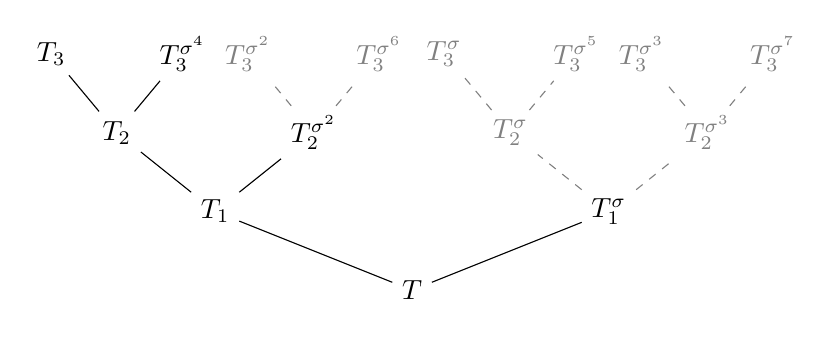
\begin{tikzpicture}
    \begin{scope}
      [level distance=1cm,
      level/.style={sibling distance=5cm/#1},
      nc/.style={gray}]
      \node{$T$}[grow'=up]
      child {node {$T_1$}
        child {node {$T_2$}
          child {node {$T_3$}}
          child {node {$T_3^{\sigma^4}$}}
        }
        child {node {$T_2^{\sigma^2}$}
          child[nc] foreach \l in {2,6} {node {$T_3^{\sigma^{\l}}$} edge from parent[dashed]}
        }
      }
      child {node {$T_1^\sigma$}
        child[nc] {node {$T_2^\sigma$} edge from parent[dashed]
          child[nc] foreach \l in {,5} {node {$T_3^{\sigma^{\l}}$} edge from parent[dashed]}
        }
        child[nc] {node {$T_2^{\sigma^3}$} edge from parent[dashed]
          child[nc] foreach \l in {3,7} {node {$T_3^{\sigma^{\l}}$} edge from parent[dashed]}
        }
      };
    \end{scope}
  \end{tikzpicture}
  
  \caption{The subproduct tree of $T$, in the case of a tower of
    quadratic extensions. Any generator of $\Gal(\U_3/\U_0)$ can be
    taken as $\sigma$. We gray out the nodes that the algorithm does
    not compute.}
  \label{fig:tree}
\end{figure}


Now the we have something like a subproduct tree for $T$, we proceed
as for interpolation. We compute recursively the polynomials in
$A_i\in\U_i[X]$ such that $A_i(x)=y$. We start from $A_k=y$. Suppose
$A_{i+1}$ is known, then we apply the \hyperref[todo]{Chinese
  remainder algorithm} to compute the polynomial
$P\in\U_{i+1}[X]/T_i(X)$ such that
\begin{equation}
  \label{eq:crt}
  P \equiv A_{i+1}^\sigma \bmod T_{i+1}^\sigma
  \qquad\text{for any $\sigma\in\Gal(\U_{i+1}/\U_i)$.}
\end{equation}
It is clear that $P$ is invariant under $\Gal(\U_{i+1}/\U_i)$, hence
$P\in\U_i[X]/T_i(X)$ and by \eqref{eq:crt} it is evident that
$P(x)=A_{i+1}(x)=y$, thus $P=A_i$.

We have thus succeeded in interpolating $A=A_0$, without having to
build the whole subproduct tree. A similar algorithm was already given
in \cite{enge+morain03}.


\begin{remark}
  Observe that, once the polynomials $T_i$ for $0\le i\le k$ are
  known, we have an efficient algorithm to evaluate polynomials in
  $g\in\U_0[X]$ at the point $x$: simply compute
  \begin{equation}
    \label{eq:191}
    \begin{aligned}
      g_0 &= g\bmod T_0\text{,}\\
      g_1 &= g_0\bmod T_1\text{,}\\
      \vdots\\
      g_k &= g_{k-1}\bmod T_k\text{,}\\
    \end{aligned}
  \end{equation}
  then $g_k=g(x)$. Transposing this algorithm gives a power projection
  algorithm that can be used in \alg{RUR}; by the discussion in
  Section~\ref{todo}, the transpose of this algorithm amounts to
  iteratively extend a linear recurring sequence. However, we do not
  use this method because it would not improve the overall complexity,
  as we shall show in the next section.
\end{remark}


\paragraph{Back to our problem}
It is easy to realize that, on inputs $x(P)$ and $x(P')$, the
algorithm we just gave computes $A^{(0)}$. In fact, $T^{(0)}$ is
the minimal polynomial of $x(P)$ over $\F_q$ and $A^{(0)}$ is the
unique polynomial in $\F_q[X]/T^{(0)}(X)$ that satisfies
\eqref{eq:affine-minimal}.

This can be viewed as decomposing the morphism $\iota$ of
Eq.~\eqref{eq:embed} as the chain of $\F_q$-linear isomorphisms
\begin{equation}
  \xymatrix{
    ^{\U_0[X_0]}/_{T_0(X_0)} \ar@{^{(}->}[r]^-{\iota_0} &
    \;\cdots\; \ar@{^{(}->}[r]^-{\iota_{k-1}} &
    ^{\U_k[X_k]}/_{T_k(X_k)} \ar@{^{(}->}[r]^-{\iota_k} &
    \U_k
  }
\end{equation}
defined by $\iota_k\circ\cdots\circ\iota_i(X_i) = x(P)$ for any $i$,
and then finding the preimage of $x(P')$ by inverting them one by
one.

Then, the Chinese remainder step we applied in \eqref{eq:crt} amounts
to invert $\iota_i$ by descending the lower path in the diagram below
\begin{equation}
  \xymatrix{
    ^{\U_i[X_i]}/_{T_i(X_i)} \ar@{^{(}->}[r]^-{\iota_i} \ar@{^{(}->}[d]^{\varepsilon} &
    ^{\U_{i+1}[X_{i+1}]}/_{T_{i+1}(X_{i+1})} \\
    ^{\U_{i+1}[Y]}/_{T_i(Y)} \ar@{^{(}->>}[r]^-{\gamma} &
    \bigoplus_\sigma {}^{\U_{i+1}[Y_{j}]}/_{\left(T_{i+1}\right)^\sigma(Y_{j})} \ar@{->>}[u]_{\pi}
  }
\end{equation}
where $\varepsilon$ is the canonical injection extending
$\U_i\subset\U_{i+1}$, $\gamma$ is the Chinese remainder isomorphism
and $\pi$ is projection onto the first coordinate.

Some care must be taken when $x(P)$ does not generate $\U_k$, but only
a subfield of index $2$. This happens when $c\not\in\F_q[c^2]$, and in
this case $\iota_0$ is not a field isomorphism. It is not to
difficult, however, to handle this case, as one only needs to take a
subgroup of index $2$ of $\Gal(\U_1/\U_0)$, instead of the whole
group, in the interpolation algorithm given above.


\subsection{Complexity analysis}
\label{sec:C2-AS-FI:complexity}

The two algorithms for computing $T^{(0)}$ and $A^{(0)}$ are very
similar and run in parallel. We can merge them in one unique
algorithm.

We set some notation. Let $i_0$ be the largest index such that
$\U_{i_0} = \U_1$ and let $\frac{p-1}{2r} = [\F_q[c^2]:\F_q]$.  Remark
that all the $T^{(j)}$'s have degree $\frac{\euler(p^{k-i_0+1})}{2r}$.
At each level $i\ge i_0$, it does the following

\begin{algorithm}
  \caption{Fast Interpolation}
  \begin{algorithmic}[1]
    \REQUIRE $T_{i+1},A_{i+1}\wrt\U_{i+1}[X]$.
    \ENSURE $T_i,A_i\wrt\U_i[X]$.
    \FORALL {$\sigma \in \Gal(\U_{i+1}/\U_i)$}
    \STATE\label{alg:T:gal} compute $\left(T_{i+1}\right)^\sigma$ and $\left(A_{i+1}\right)^\sigma$ using \alg{IterFrobenius};
    \ENDFOR
    \STATE\label{alg:T:prod} compute $T_i$ by Eq.\eqref{eq:minprod}
    through a \hyperref[todo]{subproduct tree};
    \STATE\label{alg:A:CRA} compute $A_i$ by Eq.\eqref{eq:crt} through
    \hyperref[todo]{Chinese Reminder Algorithm};
    \STATE\label{alg:T:push} convert $T_i$ and $A_i$ into
    elements of $\U_i[X]$ using \alg{Push-down}.
  \end{algorithmic}
\end{algorithm}

Step~\ref{alg:T:gal} is repeated $p$ times, each iteration taking
$O\bigl(p^{k-i}{\sf L}(i-i_0)\bigr) \subset O\bigl({\sf
  L}(k-i_0)\bigr)$ by Theorem~\ref{th:b-ifrob}.

Step \ref{alg:T:prod} takes $O\bigl(\Mult(p^{k-i_0+1}d/r)\log p\bigr)$
by \ref{todo} and step \ref{alg:A:CRA} has the same
complexity by \ref{todo}.

Step \ref{alg:T:push} takes $O\bigl(p^{k-i+1}{\sf L}(i-i_0)\bigr)
\subset O\bigl(p{\sf L}(k-i_0)\bigr)$.

For any $1\le i<i_0$, there is nothing to do because
$\U_{i+1}=\U_i$. Finally, when $i=0$ and $\U_1\ne\F_q$ the algorithm
is identical but step \ref{alg:T:gal} must be computed through a
generic Frobenius algorithm (using~\ref{todo}, for example) and step
\ref{alg:T:push} must use the implementation of $F_q[c]$ to make the
conversion (for example, linear algebra). In this case
step~\ref{alg:T:gal} costs
$\Theta\bigl(\frac{p^{k-i_0}}{r}\ModComp(pd)\log d \bigr)$
by~\ref{todo} and step \ref{alg:T:push} costs
$\Theta\bigl(p^{k-i_0}(pd)^2\bigr)$.

The total cost of the algorithm is then
\begin{equation*}
  \label{eq:T:complexity}
  O\left(\bigl(k-i_0\bigr)\bigl(p{\sf L}(k-i_0) + \Mult(p^{k-i_0+1}d/r)\log p\bigr) +
    \frac{p^{k-i_0}}{r}\bigl(\ModComp(pd)\log d + r(pd)^2\bigr) \right)
  \;\text{.}
\end{equation*}


\paragraph{The complete interpolation}
We compute all the $A^{(j)}$'s using this algorithm; there's
$p^{i_0-1}r$ of them. We then recombine them through a
\hyperref[todo]{Chinese remainder algorithm} at a cost of
$O\bigl(\Mult(p^kd)\log p^{i_0-1}r\bigr)$. The total cost of the whole
interpolation phase is then
\begin{equation*}
  O\left(\bigl(k-i_0\bigr) \bigl(p{\sf L}(k) + \Mult(p^kd)\log p\bigr) +
    p^{k-1}\ModComp(pd)\log d + p^{k-1}r(pd)^2 + i_0\Mult(p^kd)\log p
  \right)
  \;\text{,}
\end{equation*}
that is
\begin{equation}
  \label{eq:interp}
  O\left(p{\sf L}(k)\log\left(\frac{\ell}{p^{i_0}}\right) + 
    \Mult(\ell d)\log\ell\log p +
    \frac{\ell}{p}\ModComp(pd)\log d +
    \ell (pd)^2
  \right)
  \;\text{.}
\end{equation}

Alternatively, once $A^{(0)}$ is known, one could compute the other
$A^{(j)}$'s using modular composition with the multiplication maps of
$E$ and $E'$ as suggested in \cite{couveignes96}. However this
approach doesn't give a better asymptotic complexity because in the
worst case $A^{(0)}=A$. From a practical point of view, though,
Brent's and Kung's algorithm for modular
composition~\cite{brent+kung}, despite having a worse asymptotic
complexity, could perform faster for some set of parameters. We will
discuss this matter in Section~\ref{sec:C2-AS-FI-MC}.

If more than $\euler(p^k)/2$ points are needed, but less than
$\frac{p-1}{2}$, one can use the previous algorithm to interpolate
over the primitive $p^i$-torsion points for each $i=1,\ldots,k$. The
interpolating polynomials can then be recombined through a
\hyperref[todo]{Chinese remainder algorithm} at a cost of
$O\bigl(\Mult(p^kd)\log p^k\bigr)$, which doesn't change the overall
complexity of C2-AS-FI.


Putting together the complexity estimates of C2-AS and C2-AS-FI, we
have the following theorem.

\begin{theorem}
  \label{th:complexity}
  Assuming $\Mult(n) = n\log n\log\log n$, the algorithm C2-AS-FI has
  worst case complexity
  \begin{equation*}
    \tildO_{p,d,\log\ell}\left(
      p^2d^3 +
      \ModComp(p)pd +
      (pd)^\omega\log^2\ell +
      p^3\ell^2 d\log^3\ell + 
      p^2\ell^2 d^2+
      \left(\frac{\ell^2}{p} + p\right)\ModComp(pd)
    \right)
    \;\text{.}
  \end{equation*}
\end{theorem}



% Local Variables:
% mode:flyspell
% ispell-local-dictionary:"american"
% mode:TeX-PDF
% TeX-master: "../these"
% mode:reftex
% End:
%
% LocalWords:  Schreier Artin pseudotrace Frobenius bivariate Joux Sirvent FFT
% LocalWords:  Couveignes isogenies Schoof isogeny cryptosystems Lercier moduli
% LocalWords:  precomputation arithmetics polylogarithmic Karatsuba embeddings
% LocalWords:  irreducibility
